\documentclass[tikz,border=3pt]{standalone}
\usepackage[utf8]{inputenc}
\usepackage[T1]{fontenc}
\usepackage{lmodern}
\renewcommand{\familydefault}{\sfdefault}
\usepackage{sansmath}\sansmath
\usepackage{chemfig}
\usepackage{pgfplots}\pgfplotsset{compat=1.18,/pgf/number format/use comma,/pgf/number format/1000 sep={.}}
\usetikzlibrary{arrows.meta,calc,positioning,decorations.pathmorphing,patterns}
% paleta del sitio
\definecolor{nar}{HTML}{E8680C}\definecolor{narc}{HTML}{FFB35C}\definecolor{hielo}{HTML}{FFF3E8}
\definecolor{tinta}{HTML}{1D1D1F}\definecolor{gris}{HTML}{6E6E73}\definecolor{lila}{HTML}{7C5CF0}
\definecolor{azul}{HTML}{2F6FD6}\definecolor{menta}{HTML}{17A673}\definecolor{coral}{HTML}{E8342A}
\begin{document}
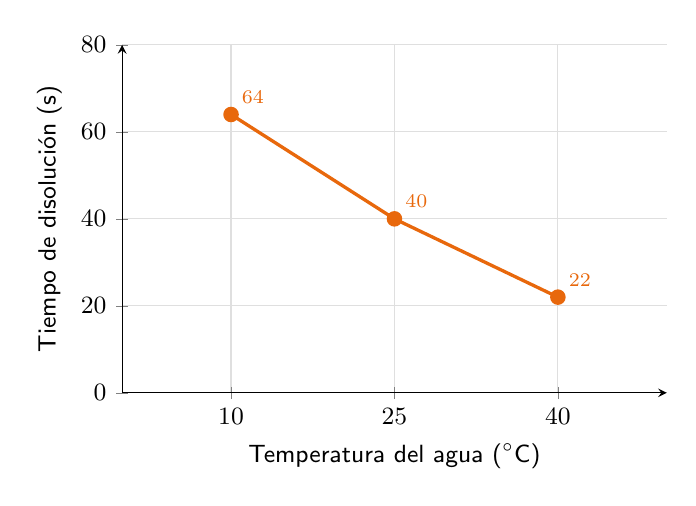
\begin{tikzpicture}[font=\small]
\begin{axis}[width=8.5cm,height=6cm,axis lines=left,xmin=0,xmax=50,ymin=0,ymax=80,xtick={10,25,40},ytick={0,20,40,60,80},
  grid=major,grid style={gray!25},xlabel={Temperatura del agua ($^\circ$C)},ylabel={Tiempo de disolución (s)},nodes near coords,
  every node near coord/.append style={font=\scriptsize\bfseries,text=nar,anchor=south west}]
\addplot[nar,very thick,mark=*,mark options={fill=nar,scale=1.1}] coordinates {(10,64)(25,40)(40,22)};
\end{axis}
\end{tikzpicture}
\end{document}
